\chapter{Design}
\label{chap:design}

\section{Design Goals}

The design is guided by several principles, roughly in order of priority:

\begin{description}[style=nextline, leftmargin=0pt]
    \item[Correctness] The hybrid handshake must produce the same session keys at both endpoints and must fail securely if either component KEM fails. The correctness of the X25519 component is inherited from the existing BoringTun implementation.
    
    \item[Security] The hybrid construction must be secure against a quantum adversary as long as at least one of X25519 or ML-KEM-768 remains unbroken. It must preserve all existing WireGuard security properties: session-key secrecy, perfect forward secrecy, replay resistance, and DoS resistance.
    
    \item[Compatibility] The implementation should coexist with unmodified WireGuard peers where possible. The PSK-slot baseline achieves this by design. The full hybrid requires protocol-level negotiation or explicit configuration of both parties to use the hybrid mode.
    
    \item[Deployability] The implementation should run on BoringTun without kernel modifications, enabling deployment on any platform that supports userspace WireGuard, including embedded and IoT devices.
    
    \item[Performance] The overhead of ML-KEM operations should not dominate handshake latency at typical network speeds. Performance on Raspberry Pi 5 is treated as the binding constraint for constrained hardware.
\end{description}

\section{The PSK-Slot Baseline}

The PSK-slot approach is the minimal intervention: a standalone binary performs ML-KEM-768 key encapsulation between two peers, derives a 256-bit shared secret, and injects it into BoringTun's preshared\_key field. After that, the WireGuard handshake proceeds exactly as in the vanilla case.

Before any WireGuard session is established, the two peers run the PSK exchange out-of-band. One peer generates an ML-KEM-768 keypair and sends the encapsulation key to the other. That peer runs ML-KEM.Encaps, obtaining a ciphertext ct and a 32-byte shared secret K, then sends ct back. The first peer runs ML-KEM.Decaps to recover the same K. Both peers configure their WireGuard interface with preshared\_key = K.

\begin{figure}[!htbp]
    \centering
    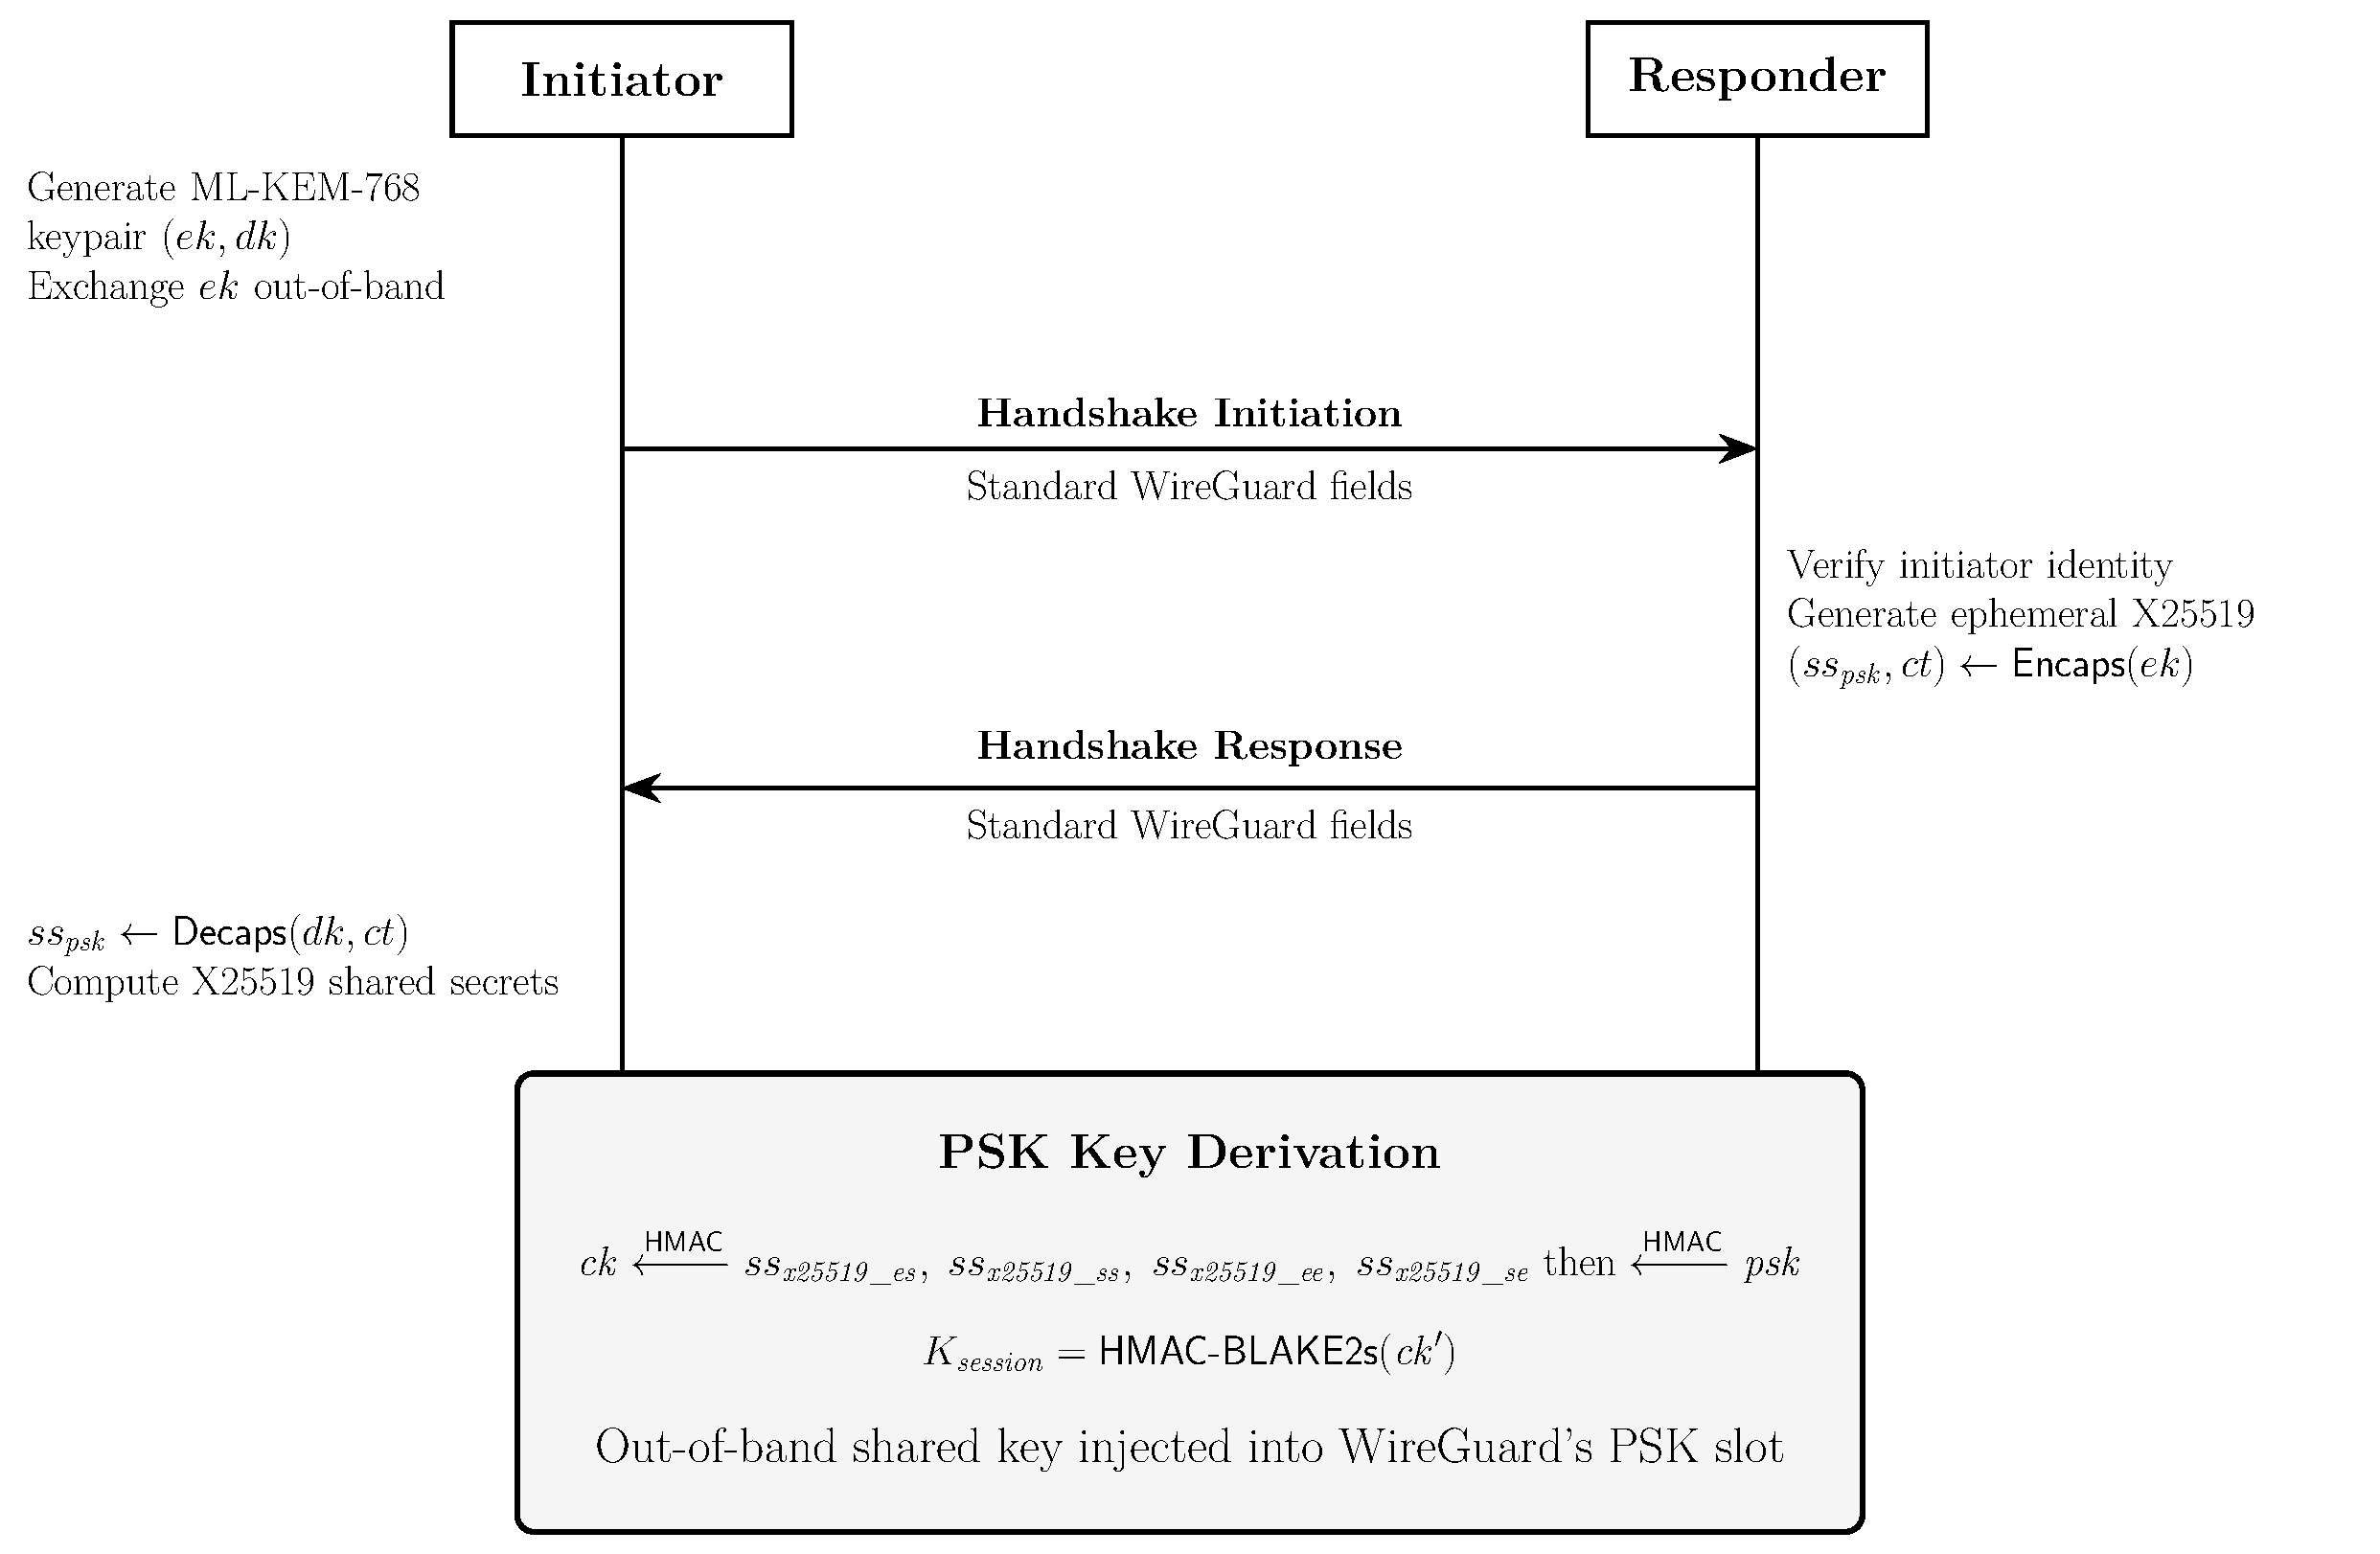
\includegraphics[width=\textwidth]{figures/fig_psk_handshake.pdf}
    \caption{PSK-Slot Baseline: Out-of-band ML-KEM exchange and PSK injection.}
    \label{fig:psk_handshake}
\end{figure}

The PSK is then mixed into the WireGuard handshake's HMAC-BLAKE2s key derivation chain, providing a quantum-resistant layer of security for all traffic protected by sessions using that PSK.

This approach has real limitations. The ML-KEM keypair used in the out-of-band exchange is static or semi-static, it does not change per handshake, so the ML-KEM component provides no forward secrecy. If the PSK is compromised after the session, all traffic from sessions that used it is exposed. The PSK also has to be distributed before any sessions can be established, which adds operational overhead.

That said, the PSK baseline has a clear advantage: it requires zero changes to WireGuard itself. It works with any existing WireGuard implementation and can be deployed immediately, providing protection against HNDL adversaries who cannot compromise the out-of-band channel.

\section{The Hybrid Handshake}

The full hybrid integrates ML-KEM-768 directly into the Noise IK handshake. The design follows the concatenate-then-KDF pattern endorsed by NIST SP 800-56C Rev.~2~\cite{nist-sp800-56c} and is structurally similar to the hybrid constructions in TLS 1.3~\cite{ietf-tls-hybrid-design}.

The modified handshake proceeds as follows:

\begin{description}[style=nextline, leftmargin=0pt]
    \item[Initiator Actions (First Message)]
    The initiator generates an ephemeral X25519 keypair as in standard WireGuard. Additionally, it generates a fresh ML-KEM-768 keypair for this session: an encapsulation key $\mathit{ek}_i$ and decapsulation key $\mathit{dk}_i$. The ML-KEM encapsulation key $\mathit{ek}_i$ (1,184 bytes) is appended to the initiator's first message, after the existing WireGuard fields. The initiator sends:
    
    \bigskip
    \begin{center}
        WireGuard initiator header, \\
        X25519 ephemeral pk, \\
        encrypted static pk, \\
        encrypted timestamp, \\
        ML-KEM-768 ek, \\
        MAC1, \\
        MAC2
    \end{center}
    \bigskip

    The ML-KEM encapsulation key is placed before the MAC fields so that MAC1 and MAC2 cover the entire message, including the ML-KEM material. This ensures that the DoS-resistance properties of the cookie mechanism extend to the post-quantum payload.

    \item[Responder Actions (Second Message)]
    The responder processes the X25519 portion of the handshake as in standard WireGuard. It also reads the initiator's ML-KEM encapsulation key $\mathit{ek}_i$ from the first message. The responder runs $\mathsf{ML\text{-}KEM.Encaps}(\mathit{ek}_i)$, producing a ciphertext $\mathit{ct}$ (1,088 bytes) and a shared secret $\mathit{ss}_\mathit{kem}$. The ciphertext $\mathit{ct}$ is appended to the responder's second message:

    \bigskip
    \begin{center}
        WireGuard responder header, \\
        X25519 ephemeral pk, \\
        encrypted empty payload, \\
        ML-KEM-768 ct, \\
        MAC1, \\
        MAC2
    \end{center}
    \bigskip

    \item[Initiator Decapsulation]
    The initiator reads $\mathit{ct}$ from the responder's message and runs $\mathsf{ML\text{-}KEM.Decaps}(\mathit{dk}_i,\allowbreak \mathit{ct})$, recovering $\mathit{ss}_\mathit{kem}$. Both peers now hold the same $\mathit{ss}_\mathit{kem}$.
    
    \item[Combined Key Derivation]
    Both parties derive the final session keys by sequentially mixing each shared secret into the Noise chaining key $\mathit{ck}$ via HMAC-BLAKE2s, following the same pattern used by standard WireGuard for its DH results. The four X25519 shared secrets from the Noise IK pattern ($\mathit{ss}_\mathit{x25519\_es}$, $\mathit{ss}_\mathit{x25519\_ss}$, $\mathit{ss}_\mathit{x25519\_ee}$, $\mathit{ss}_\mathit{x25519\_se}$, in that order) are mixed first, exactly as in vanilla WireGuard. Then the ML-KEM shared secret $\mathit{ss}_\mathit{kem}$ is mixed into $\mathit{ck}$ as an additional step:
    \[
        \mathit{temp} = \mathsf{HMAC\text{-}BLAKE2s}(\mathit{ck}, \mathit{ss}_\mathit{kem}), \quad
        \mathit{ck}' = \mathsf{HMAC\text{-}BLAKE2s}(\mathit{temp}, \mathtt{0x01})
    \]
    This sequential mixing is structurally equivalent to the concatenate-then-KDF pattern from NIST SP 800-56C Rev.~2: each shared secret contributes independently to the chaining key, and the final session keys depend on all components. The handshake hash $h$ is also updated to include the ML-KEM material (both the encapsulation key and ciphertext), binding it to the Noise transcript.
    
    \item[Transport Phase]
    After key derivation, the data transport phase proceeds identically to unmodified WireGuard. No changes are required to the ChaCha20-Poly1305 transport encryption or the session management layer.
    \end{description}

    \begin{figure}[!htbp]
    \centering
    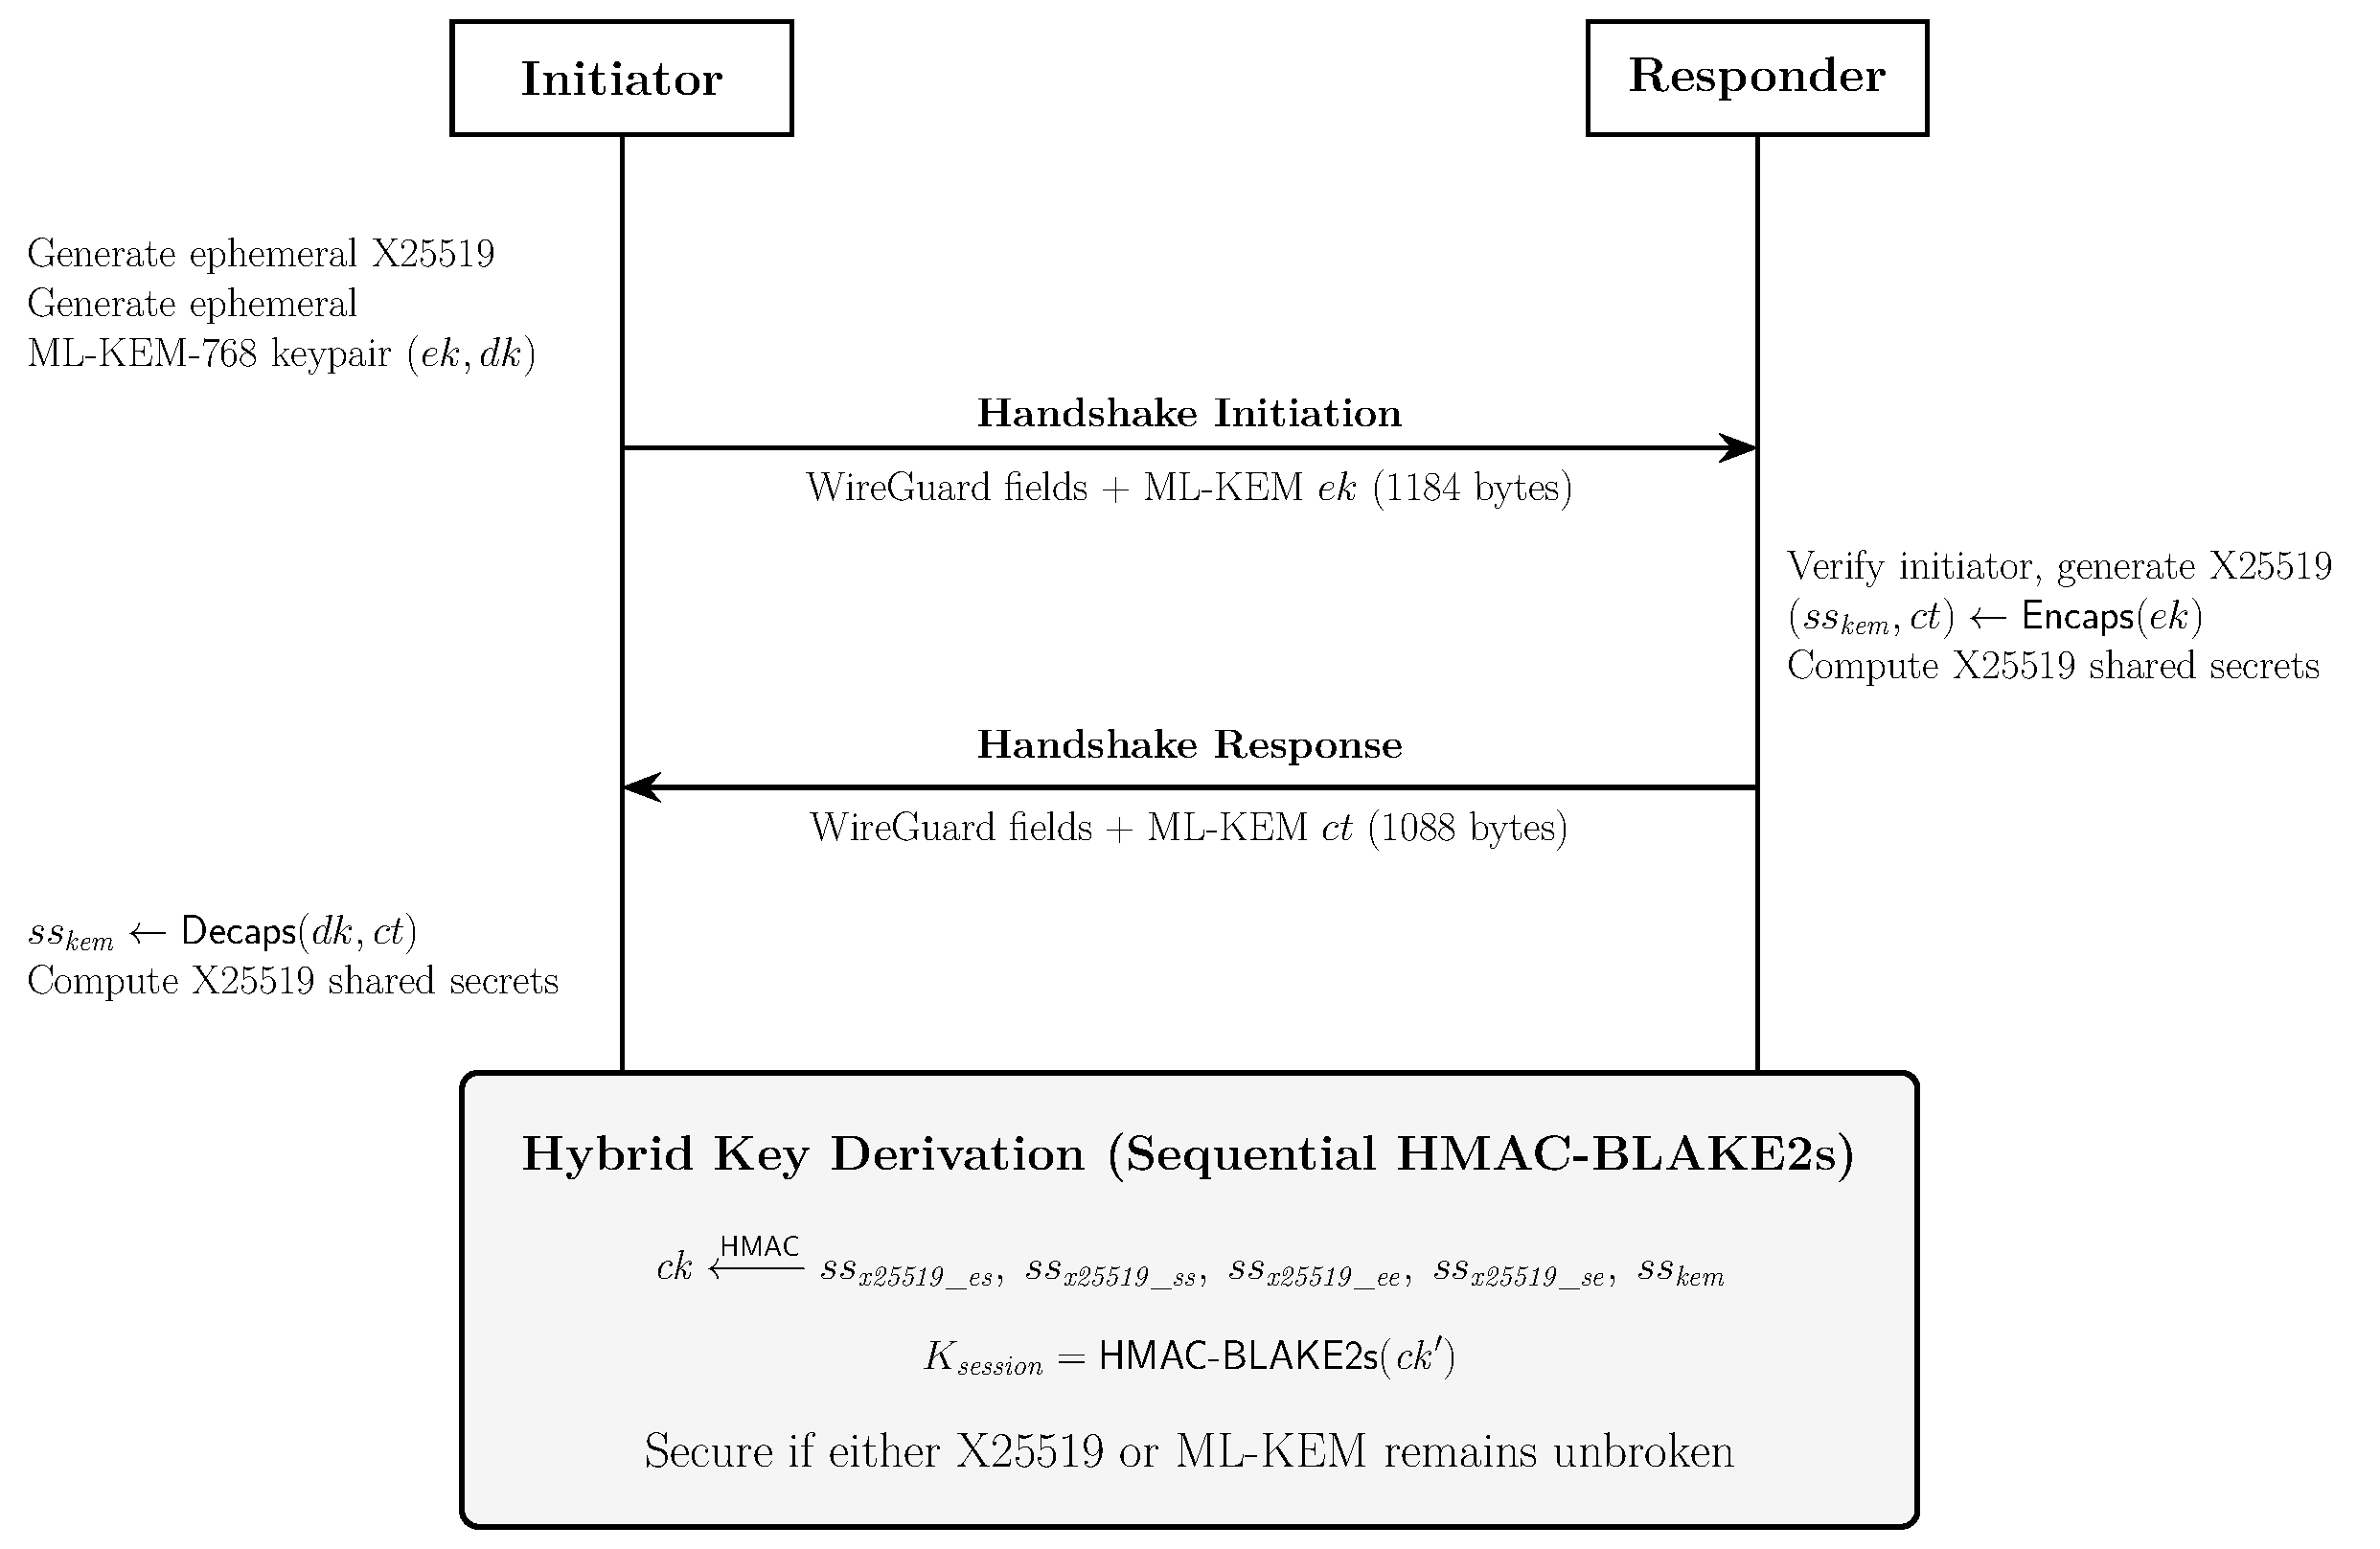
\includegraphics[width=\textwidth]{figures/fig_hybrid_handshake.pdf}
    \caption{The Full Hybrid Handshake: Integrated ML-KEM-768.}
    \label{fig:hybrid_handshake}
    \end{figure}

    Two properties follow from this design.
 Per-session forward secrecy comes from both components: the X25519 ephemeral key is fresh for each handshake, and so is the ML-KEM keypair, making $\mathit{ss}_\mathit{kem}$ unique to each session. The construction is also \emph{hybrid-secure}: if ML-KEM is completely broken (an adversary knows $\mathit{ss}_\mathit{kem}$), the session key still depends on the X25519 exchange and cannot be recovered without breaking X25519 too. The converse also holds: a quantum adversary who breaks X25519 still cannot derive the session key without also breaking ML-KEM.

\section{Key Derivation Details}

The key derivation in the hybrid handshake extends the Noise IK chaining key evolution with one additional mixing step for the ML-KEM shared secret. The approach is structurally consistent with the concatenate-then-KDF pattern from NIST SP 800-56C Rev.~2~\cite{nist-sp800-56c}, adapted to the sequential HMAC-based mixing used by the Noise Protocol Framework.

In the standard WireGuard Noise IK handshake, the chaining key $\mathit{ck}$ evolves through a sequence of HMAC-BLAKE2s mixing operations as shared secrets are established. Each DH result is mixed into $\mathit{ck}$ via a two-step HMAC extraction:
\[
    \mathit{temp} = \mathsf{HMAC\text{-}BLAKE2s}(\mathit{ck}, \mathit{ss}), \quad
    \mathit{ck} \leftarrow \mathsf{HMAC\text{-}BLAKE2s}(\mathit{temp}, \mathtt{0x01})
\]

In the hybrid, the ML-KEM shared secret $\mathit{ss}_\mathit{kem}$ is mixed into the chaining key after the X25519 DH operations and before the PSK mixing step. Concretely:

\begin{enumerate}
    \item The standard Noise IK chaining key derivation proceeds: $\mathit{ck}$ is updated with the four X25519 DH results from the IK pattern --- $\mathit{ss}_\mathit{x25519\_es}$ (ephemeral-static), $\mathit{ss}_\mathit{x25519\_ss}$ (static-static), $\mathit{ss}_\mathit{x25519\_ee}$ (ephemeral-ephemeral), and $\mathit{ss}_\mathit{x25519\_se}$ (static-ephemeral) --- each via the HMAC-BLAKE2s extraction above, exactly as in standard WireGuard. One detail worth noting: BoringTun caches $\mathit{ss}_\mathit{x25519\_ss}$ as \texttt{NoiseParams.static\_shared} when a peer is first added and reuses it across handshakes. The value is still mixed into $\mathit{ck}$ every time, but only the other three DH results are recomputed per handshake, so the per-handshake cost across both peers comes out at six fresh DH operations rather than eight (see Section~\ref{sec:handshake_latency_results}).

    \item An additional HMAC-BLAKE2s mixing step incorporates $\mathit{ss}_\mathit{kem}$:
    \[
        \mathit{temp} = \mathsf{HMAC\text{-}BLAKE2s}(\mathit{ck}, \mathit{ss}_\mathit{kem}), \quad
        \mathit{ck}' = \mathsf{HMAC\text{-}BLAKE2s}(\mathit{temp}, \mathtt{0x01})
    \]
    The ML-KEM ciphertext is also mixed into the handshake hash: $h \leftarrow \mathsf{BLAKE2s}(h \| \mathit{ct})$, binding it to the Noise transcript.

    \item The PSK mixing step proceeds on $\mathit{ck}'$ exactly as in standard WireGuard (using a zero PSK if none is configured).

    \item The final session key pair ($\mathit{send\_key}$, $\mathit{recv\_key}$) is derived from the resulting chaining key as in standard WireGuard.
\end{enumerate}

BLAKE2s is used throughout: for the handshake hash $h$, and as the PRF underlying the HMAC-based key derivation chain. This is consistent with BoringTun's existing implementation and with the WireGuard protocol specification. No SHA-256 or separate HKDF construction is introduced; the hybrid extension reuses the same HMAC-BLAKE2s extraction pattern already used for the X25519 shared secrets.

\section{Message Size Analysis and MTU Considerations}

The biggest practical challenge with the hybrid handshake is the increased message size. Vanilla WireGuard's handshake initiation message is 148 bytes and the response is 92 bytes (accounting for all headers, encrypted fields, and MACs). Adding ML-KEM-768 material adds 1,184 bytes to the initiation message (the encapsulation key) and 1,088 bytes to the response message (the ciphertext). The total handshake message sizes become approximately 1,332 bytes for the initiation and 1,180 bytes for the response.

The IPv6 minimum MTU is 1,280 bytes. Both hybrid handshake messages exceed this threshold. The IPv4 minimum MTU is 68 bytes (though in practice the de facto minimum for internet paths is 576 bytes), and typical deployed MTUs are 1,500 bytes for Ethernet.

This creates a fragmentation problem. WireGuard transmits handshake messages as UDP datagrams. Unlike TCP, UDP does not have a built-in fragmentation and reassembly mechanism at the application layer; IP-level fragmentation may occur, but it is unreliable on many real-world network paths (some firewalls drop fragments), and it reduces resilience.

The current implementation relies on IP-level fragmentation to handle oversized handshake messages. On typical Ethernet paths with a 1,500-byte MTU, the initiation message (1,332 bytes) fits in a single UDP datagram without fragmentation. The response message (1,180 bytes) also fits comfortably. On paths with a reduced MTU (e.g., the IPv6 minimum of 1,280 bytes), the initiation message will be fragmented at the IP layer. This approach is the simplest and works correctly on network paths that do not drop fragments.

For deployments on paths where IP fragmentation is unreliable (e.g., certain firewall configurations or middleboxes that drop fragments), two alternative strategies are identified as future work:

\begin{description}[style=nextline, leftmargin=0pt]
    \item[Application-Level Segmentation]
    Split the handshake messages at the application layer, sending the ML-KEM material in a separate UDP datagram. This requires a protocol extension and adds an additional round trip for ML-KEM key material exchange.

    \item[Path MTU Discovery with KEM Parameter Negotiation]
    Use PMTUD to discover the path MTU before the handshake and choose a KEM parameter set whose ciphertext fits within the available space. For most internet paths with a 1,500-byte MTU, ML-KEM-768 fits comfortably; for IPv6 paths requiring sub-1,280-byte packets, a reduced parameter set or segmentation would be needed.
\end{description}

These strategies are not implemented in the current version of the hybrid handshake. On standard 1,500-byte MTU paths the IP-level approach already does the job, and a proper quantitative study of how the hybrid behaves on constrained paths is left as future work.
